\documentclass[12pt]{report}
\usepackage{listings}
\usepackage{underscore}
\usepackage{vhistory}
\usepackage{setspace}
\usepackage{listings}
\usepackage{xparse}
\usepackage{xcolor}
\usepackage{mhchem}


\definecolorset{rgb/hsb/cmyk/gray}{}{}%
 {red,1,0,0/0,1,1/0,1,1,0/.3;%
  green,0,1,0/.33333,1,1/1,0,1,0/.59;%
  blue,0,0,1/.66667,1,1/1,1,0,0/.11;%
  brown,.75,.5,.25/.083333,.66667,.75/0,.25,.5,.25/.5475;%
  lime,.75,1,0/.20833,1,1/.25,0,1,0/.815;%
  orange,1,.5,0/.083333,1,1/0,.5,1,0/.595;%
  pink,1,.75,.75/0,.25,1/0,.25,.25,0/.825;%
  purple,.75,0,.25/.94444,1,.75/0,.75,.5,.25/.2525;%
  teal,0,.5,.5/.5,1,.5/.5,0,0,.5/.35;%
  violet,.5,0,.5/.83333,1,.5/0,.5,0,.5/.205}%
\definecolorset{cmyk/rgb/hsb/gray}{}{}%
 {cyan,1,0,0,0/0,1,1/.5,1,1/.7;%
  magenta,0,1,0,0/1,0,1/.83333,1,1/.41;%
  yellow,0,0,1,0/1,1,0/.16667,1,1/.89;%
  olive,0,0,1,.5/.5,.5,0/.16667,1,.5/.39}
\definecolorset{gray/rgb/hsb/cmyk}{}{}%
 {black,0/0,0,0/0,0,0/0,0,0,1;%
  darkgray,.25/.25,.25,.25/0,0,.25/0,0,0,.75;%
  gray,.5/.5,.5,.5/0,0,.5/0,0,0,.5;%
  lightgray,.75/.75,.75,.75/0,0,.75/0,0,0,.25;%
  white,1/1,1,1/0,0,1/0,0,0,0}



\usepackage[bookmarks=true]{hyperref}
\usepackage{graphicx}
\graphicspath{ {./images/} }
\hypersetup{
    pdftitle={Software Requirement Specification},    % title
    pdfauthor={Yiannis Lazarides},                     % author
    pdfsubject={TeX and LaTeX},                        % subject of the document
    pdfkeywords={TeX, LaTeX, graphics, images}, % list of keywords
    colorlinks=true,       % false: boxed links; true: colored links
    linkcolor=blue,       % color of internal links
    citecolor=black,       % color of links to bibliography
    filecolor=black,        % color of file links
    urlcolor=purple,        % color of external links
    linktoc=page            % only page is linked
}%

\usepackage{geometry}
\geometry{margin=1.5in}
\onehalfspacing


\usepackage{atbegshi}% http://ctan.org/pkg/atbegshi
\AtBeginDocument{\AtBeginShipoutNext{\AtBeginShipoutDiscard}}


\title{%




\Huge{Követelményelemzés}\\
\vspace{2cm}

Marsjáró jármű\\
\vspace{2cm}

\LARGE{Verzió 1.0}
\vspace{2cm}

\small{
Készítették:\\
Cseresnyés Kristóf: @aPisC\\
Fikó Róbert: @robertfiko\\
Gőgös Márton: @Marzyh\\
Hosek Henrietta: @hosekhenrietta\\
Kurucz Ádám: @engreyight\\
Lippa Katalin: @katilippa\\
Miskolczi Péter: @BreadKingGod\\
Monhor Hubert: @dopamean\\
Novák-Schwartz József: @JNSchwartz\\
Szabó Tihamér: @SzaboTihi14\\
Szerednik László Tamás: @szeredniklaszlo\\
}
}
\date{}
\usepackage{hyperref}



\begin{document}


\newcommand{\reqid}[1]{\colorbox{lightgray}{#1}}
%\newcommand{\reqidc}[2]{
%  \colorbox{lightgray}{#1_\arabic{#2}}
%}
\maketitle

\tableofcontents
\begin{versionhistory}
  \vhEntry{1.0}{22.10.23}{Novák-Schwartz József}{1st revision}
  \vhEntry{1.1}{22.11.06}{Robert Fiko}{Subsystems, risk analysis and formatting}
  \vhEntry{1.2}{22.11.09}{BreadKingGod}{Meghajtas}
  \vhEntry{1.3}{22.11.11}{szerendiklaszlo}{Navigation, sensors}
  \vhEntry{1.4}{22.11.12}{engreyight}{Drill}
  \vhEntry{1.5}{22.11.12}{szabotihi}{Supply, food, drink}
  \vhEntry{1.6}{22.11.12}{Novák-Schwartz József}{Spacesuit}
  \vhEntry{1.6.1}{22.11.13}{Robert Fiko}{Merge and review}
  \vhEntry{1.6.2}{22.11.13}{engreyight}{Glossary}
  \vhEntry{1.7}{22.11.13}{apisc}{Strength requirements}
  \vhEntry{1.8}{22.11.13}{katilippa}{Repairablity and upgradability}
  \vhEntry{1.9}{22.11.20}{BreadKingGod}{Meghajtas 2.0}
  \vhEntry{1.9}{22.11.20}{dopamean}{Komfort}
  \vhEntry{1.9.1}{22.11.13}{Robert Fiko}{Merge and review}



  

\end{versionhistory}
\chapter{Projekt bemutatása}
A NASA a Mars emberekkel történő felfedezéséhez magáncégek pályázatát várja a szükséges hardver és szoftverelemek kifejlesztéséhez az alábbi témakörökben:
\begin{enumerate}
  \item Marsbázis
  \item \textbf{Marsjáró jármű}
  \item Ellátmányűrhajó
  \item Mars-járó jármű
\end{enumerate}

Ebben a projektben 2 Mars-járó járműre készítünk specifikációt az alábbiakat figyelembe véve:
\begin{itemize}
  \item A járműveknek maximum 4 ember ellátását kell biztosítaniuk a Mars-járó missziók
időtartamára
  \item A jármű élettartama minimum 5 év legyen a Marsi körülmények között
  \item A járműnek lehetőséget kell biztosítania az űrhajósok kiszállására és beszállására
közvetlenül a Marsra vagy a marsi bázisra
  \item A jármű képes legyen a misszióhoz szükséges segédfelszerelések szállítására, vizsgálatok
elvégzésére, valamint a begyűjtött kőzetminták szállítására
  \item Az eszközhöz csatlakozzon egy repülni képes, felderítő drón
  \item A járműnek képesnek kell lennie kommunikálnia a Marsbázissal és a Mars körül keringő
átjátszó műholdakkal valamint űrállomással
  \item Végezzen kockázatanalízist és a szükséges alrendszereknél alkalmazzon redundanciát
  \item A főbb alrendszereknek javíthatónak és cserélhetőnek kell lennie az ellátmány bázis
alkatrészei alapján
\end{itemize}

\chapter{Követelmények}
\section{Követelmények számozása és rendszere}
A követelmények egyedi azonosítására az alábbi formátumot használjuk \\ 
\textbf{A_ID}, ahol \textbf{A} annak a részterületnek az azonosítója, ahova a követelmény tartozik, \textbf{ID} pedig az azon belüli követelmény azonosító.

\subsection{Alkategóriák, részterületek}
\begin{itemize}
  \item \reqid{NS}: navigáció és szenzorok követelményei 
  \item \reqid{F}: fúró követelményei
  \item \reqid{R}: robotkar követelményei
  \item \reqid{S}: szenzorok követelményei
  \item \reqid{M}: meghajtás követelményei
  \item \reqid{Z}: szkafander, űrruha követelményei
  \item \reqid{D}: drón követelményei
  \item \reqid{H}: humán követelmények
  \item \reqid{L}: telekommunkációs követelmények
  \item \reqid{CS}: csatlakozási követelmények
  \item \reqid{D}: drón követelmények
  \item \reqid{K}: kutatási követelmények
  \item \reqid{J}: javíthatósági követelmények
  \item \reqid{T}: strapabírósági követelmények
  \item \reqid{KO}: komfort követelmények
	  
  \item \reqid{U}: utókövetelmények
\end{itemize}




\section{Megvalósítás ütemterve}

A megvalósítás ütemtervet, a marsbázis csapattal egyeztetve, az alábbiak szerint állítottuk fel.

\begin{itemize}
  \item Tervezési fázis: 2025. május 10
  \begin{itemize}
    \item A jármű részletes terveinek el kell készülnie.
  \end{itemize}
  \item Első prototípus: 2028. május 10
  \begin{itemize}
    \item Alapvető motorikus funkciók
    \item Dokkolás, légzsilip
    \item kommunikáció
    \item robot kar
  \end{itemize}
  \item Második prototípus: 2030. május 10
  \begin{itemize}
    \item Kisebb hibák még elfogadhatóak
    \item A véglesges specifikációt be kell tartalékmoduljainak
    \item Legalább 95\%-ban legyen megvalósítva
  \end{itemize}
  \item Tesztelés a Földön: 2031. május 10
  \begin{itemize}
    \item sarkvidéki, sivatagi és vulaknikus körülmények között
  \end{itemize}
  \item Marsi leszállítás: 2035. május 10
\end{itemize}


\section{Mérnöki követelmények}
\begin{itemize}
  \item A marsjáró mérete 8 m * 5 m * 3.5 m (Hosszúság * Szélesség * Magasság).
  \item A marsjáró kereke a ref{drive} fejezetben van definiálva \
  \item A marsi körülményeknek ellenálló anyag, védőréteg (\ref{strapabirosag} alapján)
\end{itemize}

\subsection{A jármű alrendszerei}\label{subsystems}

A biztonságos és megbízható működés, illetve a modularitás elveinek betartása végett a 
járművet alrendszerekre bontjuk.

\subsubsection{Navigáció és szenzorok}
A navigációs alrendszer célja a vezetőt ellátni információkkal a terepviszonyokról, útvonalat tervezni a marsi felszínen, illetve egy bizonyos szintű önvezetést megvalósítani.

\noindent\textbf{Szükséges moduláris érzékelők és eszközök}
\begin{itemize}
  \item \reqid{NS_1} műholdas antennák
  \item \reqid{NS_2} giroszkóp és gyorsulásmérő
  \item \reqid{NS_3} motorhő-érzékelő
  \item \reqid{NS_4} több irányba tekintő ultrahangos szenzorok és közelség- és mélységérzékelők
  \item \reqid{NS_5} 360 fokos és 3D térlátást biztosító nagy felbontású kamerák 
  \item \reqid{NS_6} számítógépes egység (az adatok feldolgozásához)
\end{itemize}

\noindent\textbf{Biztosított funkciók}
\begin{itemize}
  \item \reqid{NS_7} helyzetmeghatározás: antennák által az űrbázis marsi műholdjaira csatlakozva
  \item \reqid{NS_8} térkép felépítése: műholddal készült felvételekkel, marsjáró által már bejárt helyekről készült adatrögzítés által
  \item  \reqid{NS_9} környezetfelismerés: akadálymentes meghajtás szenzorok és kamerák által \begin {itemize}
      \item lehetséges-e a kívánt dőlésszögben való haladás
      \item megléphetetlen akadályok detektálása
    \end{itemize}
\end{itemize}

\noindent\textbf{Különleges irányelvek}
\begin{itemize}
  \item alacsony üzemanyagszint: energiahasználat csökkentése a nem szükséges szenzorok kikapcsolásával, ezáltal növelni az esélyét a bázisra visszatérésnek
  \item útvonalon be nem tervezett akadály: újratervezés biztonságos útvonalat keresve
\end{itemize}

Becslések, gyártás és beszerzés, valamint ezek ledelegálása:
\begin{itemize}
  \item antennák, kamerák és szenzorok beszerzése: \begin{itemize}
      \item megfelelő mennyiségű éles- és tartalékkészlet megrendelése
      \item kapcsolatfelvétel az elvárt minőséget biztosító, és minél kedvezőbb árat kiszabó beszállítókkal
      \item időbecslés: 1.5 hónap
      \item pénzbecslés: 350 AK
    \end{itemize}
  \item \reqid{NS_10} navigációs szoftver: \begin{itemize}
      \item előfeltétel: navigációs szenzorok beszerzése, programot elkészítő csapat megbízása
      \item időigény: 6 hónap
      \item pénzbecslés: 10000 AK
    \end{itemize}
  \item összesített becslés: \begin{itemize}
      \item előfeltétel: navigációs szenzorok beszerzése, programot elkészítő csapat megbízása
      \item időigény: 7.5 hónap
      \item pénzbecslés: 10350 AK
    \end{itemize}
\end{itemize}

Ahol 1 Arany Krajcár (AK) = 1 EUR

\subsubsection{A fúró és szenzorai, vizsgálatok}

A marsjárónak több különböző fúrófejjel kell rendelkeznie, melyek cserélhetők. Ezeket használja egyrészt 30 cm mély lyukak fúrására (\reqid{F_1}), illetve a felszín lekaparására. (\reqid{F_2}) Az így keletkezett lyukak alján ezután párologtatást (\reqid{F_3}) végez, és az így kiváló anyagokat összegyűjti. (\reqid{F_4}) Emellett képes a felszínen már jelenlévő és a kaparással előállított regolitot felszívni, illetve esetlegesen maximum 50x25x25cm-es már szabadon lévő kőzetdarabokat begyűjteni. (\reqid{F_5})  A marsjáró összesen 800kg kőzetminta tárolására és szállítására képes. (\reqid{F_6}) 

A minták tárolására két fajta tároló használható. Egy egyszer használatos, melyet a minták felhasználása után ki kell dobni, vagy egy speciális, vegyszeres tisztítás után újrahasznosítható. Szükség van emelett olyan "tárolókra", amelyekbe nem kerülnek minták, csupán arról adnak tanubizonyságot, hogy a kinyerés során nem szennyeződött a többi minta. (\reqid{F_7}) 

A fúró egy robotkarra van rögzítve, mely számos szabadsági fokkal, vagy izülettel rendelkezik. 

Első a váll, amely minden irányban mozgatható egy megadott tartományban. (\reqid{R_1}) Ezt követi a könyök, amely hajlítható és egy 360 fokban elforgatható csukló. (\reqid{R_2}) Ennek a végén található egy fogó, melynek egyik ága a fúró, a másik pedig egy kamera, amely a fúrást segíti.  Ehhez egy lámpa is tartozik, és normál fénytartományban működik. (\reqid{R_3}) Emellett található rajta egy biztonsági kontaktszenzor, amely véd a berendezés meghibásodása ellen. (\reqid{R_4})

A marsjárón a fúrófejhez tartozó kamera mellett található még 4, ebből 2 előre, 2 pedig hátrafelé néz. Ezek kellő távolságban vannak egymástól ahhoz, hogy a mélységérzékelés működjön. Minden kamerához tartozik 1-1 lámpa, és ezek az infravörös tartományban is működnek. (\reqid{NS_11})

Az összegyűjtött mintákat el lehet tárolni, és a bázisra szállítani, vagy akár már a marsjáróban fel lehet őket nyitni és alapvető vizsgálatokat végezni rajtuk.

A vizsgálatok fő célja a bolygó geológiájának és történelmének feltárása, múltbéli élhetőségének vizsgálata, és víz és sejtes élet nyomainak keresése.

\subsubsection{Egyéb szenzorok}
A marsjáró optimális külső és belső állapotainak ellenőrzéséhez szükség van a navigációtól független szenzorokra is.

Ezekhez szükségesek:
\begin{itemize}
  \item külső szenzorok: \begin{itemize}
      \item \reqid{S_1} külső hőmérő
      \item \reqid{S_2} napállást vizsgáló szenzor
      \item \reqid{S_3} légnyomásmérő
    \end{itemize}
  \item belső szenzorok: \begin{itemize}
      \item \reqid{S_4} marsjáró és szkafanderek töltöttség-mérője
      \item \reqid{S_5} oxigénszint-mérő
      \item \reqid{S_6} nyomásszint-mérő
      \item \reqid{S_7} belső hőmérő (ezáltal ellenőrizve a megrendelő által elvárt belső hőt)
      \item \reqid{S_8} kőzetminta mérleg (hogy ne lépjük túl a megrendelő által maximálisan elvártan szállított kőzetek tömegét)
    \end{itemize}
\end{itemize}

Ezek által megállapítható, hogy:
\begin{itemize}
  \item alkalmasak-e a külső körülmények a marsjáró épségben maradását tekintve
  \item alkalmasak-e a belső körülmények marsjáróban lévő emberek számára
\end{itemize}

\subsubsection{Meghajtás \label{drive}}

Komponensek:

\begin{itemize}
    \item \reqid{M_1} Kerék: 
        \begin{itemize}
            \item Levegőmentes kerék
            \item Alumíniumból kell készíteni
            \item A tapadás érdekében kapcsokkal kell rendelkeznie
            \item A rugós tapadásért titánium külőket kell bele építeni
        \end{itemize}
    \item \reqid{M_2} Futómű:
        \begin{itemize}
            \item Fémből kell készíteni
            \item Teherbírásának akkorának kell lenni, hogy elbírja a kocsi tömegét
        \end{itemize}
    \item \reqid{M_3} Motor:
        \begin{itemize}
            \item Hidrogénmotor
            \item Bázistól feltöltéskor vizet és energiát kapunk, a vizet a kapott energia segítségével kell oxigénre és hidrogénre bontani
            \item A motor belsejében a hidrogént az oxigén segítségével elégetjük, a felszabaduló energiát használja a motor meghajtásra, a melléktermék vizet meg emberi fogyasztásra alkalmazható
        \end{itemize}
    \item \reqid{M_4} Tank:
        \begin{itemize}
            \item Méretének akkorának kell, hogy 200 km üzemanyag elférjen benne
            \item Két azonos méretű üzemanyag cellából álljon
            \item A két üzemanyag cellából párhuzamosan fogyasszon üzemanyagot
            \item Az üzemanyag cellák legyenek képesek önállóan is ellátni az eszközt
            \item Feltölthető legyen a bázisról
            \item Legyen egy rendszer ami méri a tank az üzemanyagcellák töltöttségét
            \item Ez a rendszer értesítse a vezetőt, amikor a tank töltöttség félig van
            \item Az üzemanyagcellák dokkolva tölthetőnek kell lenniük
        \end{itemize}
    \item \reqid{M_5} Közlekedés:
        \begin{itemize}
            \item El kell érnie a  25 km/h sebességet
            \item Képesnek kell lennie 20 nap alatt 20 km-t megtenni
            \item A bevehető meredekségének 20-30-osnak kell lennie
            \item A járműnek képesnek kell lennie oldalazva közlekedni
        \end{itemize}
\end{itemize}

Becslések és gyártás:

\begin{itemize}
    \item Kerék:
        \begin{itemize}
            \item Beszerez:
                \begin{itemize}
                    \item Titánium küllők: Total Titan Titanium
                    \item Aluminum: Cosmo Aluminum
                \end{itemize}
            \item Gyártás: mi gyártjuk
            \item Idő becslés: 2 hónap
            \item Pénz becslés: 450 AK
        \end{itemize}
    \item Tank:
        \begin{itemize}
            \item Gyártás: delegáljuk a HCella cégnek
            \item Idő becslés: 1 hónap
            \item Pénz becslés: 100 AK
        \end{itemize}
    \item Motor:
        \begin{itemize}
            \item Gyártás: delegáljuk a Massive Motor cégnek
            \item Előfeltétel: 
                \begin{itemize}
                    \item Tank
                \end{itemize}
            \item Idő becslés: 1 év
            \item Pénz becslés: 10000 AK
        \end{itemize}
    \item Futómű:
        \begin{itemize}
            \item Beszerez:
                \begin{itemize}
                    \item Aluminum: Cosmo Aluminum
                \end{itemize}
            \item Gyártás: mi gyártjuk
            \item Előfeltétel: 
                \begin{itemize}
                    \item Motor
                    \item Kerék
                \end{itemize}
            \item Idő becslés: 6 hónap
            \item Pénz becslés: 5500 AK
        \end{itemize}
    \item Összesített:
        \begin{itemize}
            \item Idő becslés: 1 év, 9 hónap
            \item Pénz becslés: 16050 AK
        \end{itemize}
\end{itemize}

\subsubsection{Létfenntartás}

Természetesen az emberi személyzet végett, a létfenntartó rendszerek elengedhetetlenek. Vlevegő szűrő és széndioxid kivonó rendszerrel, illetve vízújrahasznosító rendszerrel fogjuk felszerelni. Az utóbbi képes a levegő páratartalmát kivonni, illetve vizeletet tisztítani, így végül fogyasztásra alkalmas ivóvizet kapunk. (ld. \reqid{H_5})

Az asztronautáknak a megfelelő hőmérséklet biztosítására fűtő berendezést szerelünk, mivel a marsi hőmörséklet nem haladja meg a 21 Celsius fokot, így fűtés biztosítása elegendő.

Forrás: https://www.weather.gov/fsd/mars


\subsubsection{Telekommunikáció}

A telekommunkációhoz 2 megabit/s adatátviteli sebességű, úgynevezett UHF antennákat fogunk használni. \reqid{L_1}

Forrás: https://descanso.jpl.nasa.gov/DPSummary/MER\_article\_cmp20051028.pdf és https://mars.nasa.gov/msl/spacecraft/rover/communication/

A marsjárók képesek egymással kommunikálni illetve a \reqid{L_2} bázissal, \reqid{L_3}űrállomással is (az ellátmányhajóval való kommunikációs kapcsolat szükségtelen)  full-duplex módon.  Ez a kommunikációs csatorna élő hang és videó kapcsolat létrehozására is képes. Ezt a járműben elhelyezett képernyő és kamera is biztosítja. A felvételeket a megrendelő kérésére tároljuk. Minimális, pár másodperces késés elfogadható a kommunikáció során.
A kommunikáció biztosított a bázis \reqid{L_3} 300 km-es távolságú sugarában.


\subsubsection{Mars járó bejáratai, csatlakozás a bázishoz}
A járón \reqid{CS_1} két bejárat található, két szemközti oldalán. 
\begin{itemize}
\item \reqid{CS_2}A mars járóból a a bolygó felszinére való kijutást biztosító zsilipes rendszerrel működtetett kapu.
\item \reqid{CS_3}A mars járóról a bázishoz való csatlakozást biztosító bejárat. A járművet a bázissal egy híd köti össze, mely mozgatható, így a vertikális egyenlőtlenségeket a bejáratok között ez hidalja át.
\end{itemize}

\reqid{CS_4}A bejáratot egy vezérlőpult irányítja.

\reqid{CS_5}A zsilip kamrájában egyszerre két ember tartózkodhat.

\reqid{CS_6}A kamra a marsi levegő szűrésén kívűl fertötlenítést is végez.
A marsjáróknak  nem kell összekapcsolódniuk egymással, átjárni egyikből a másikba.

\subsubsection{Szkafander/űrruha és a mars járó kapcsolata}
\begin{itemize}

  \item \reqid{Z_1} A bázissal megegyezö módon töltjük a szkafander elektromos akkumulátorát és oxigénpalackját is a roverben.
  \item \reqid{Z_2} A jármüvön egy fajta sürített \(O_2\) palack, amiből a járón belül is keverjük a levegöt, és a palackot is tudjuk tölteni, ezt pedig a bázison töltjük újra. Biztonsági redundancia szempontból persze lehet több palack, de praktikus, ha csak egyfajta, és mindkét funkciót képes biztosítani.
  \item \reqid{Z_3} Töltöaljzat és oxigéncsap biztosítása.
  \item \reqid{Z_4} Szkafander töltö alkatrész, oxigén palack szükítö alkatrész.
  \item Ezek beszerelése a teljes elektromos és oxigén kivitelezési körök után kezdödhet, és átadásig elég befejezödnie.
  \item \reqid{Z_5} A tiszta oxigén légzése elött egy ú.n. elölégzésre van szükség, ami a nitrogént kiüríti a szervezetböl, így megelözve a sérüléseket. Ehhez szükséges vákuumkamra biztosítása. Javaslom a mars felé nyíló zsiliprendszer vákuumképzéssel felruházását.
  \item \reqid{Z_6} Oxigén nyomás kritikus csökkenés esetén, vagy kritikus áramcsökkenés esetén azonnali visszatérés megkövetelése. Fel nem töltött szkafanderek esetén töltés azonnali megkövetelése, vagy kötelezö visszatérés. A humán biztonság megköveteli, hogy mindig legyen töltött szkafander evakuációhoz.
\end{itemize}

\subsubsection{Drón}

A marsjáróhoz tartozik egy drón. Ez egy a földön hétköznapi emberek által is használt drónhoz hasonló működési elvű eszköz. A feladata felderítés. A marsjáróhoz kapcsolódik és egy-egy misszió során gyűjt képanyagokat a környezetről.

A drón repülésre képes, ehhez két koaxiális propellerrel van felszerelve. (\reqid{D_1}) Ezek használatosak helikoptereknél is, ugyanis megkönnyítik a manőverezést. Mind a hajtásért felelős szerkezet, mind maga a drón váza és egyéb építőegységei - hasonlóan a marsjáróhoz - olyan anyagokból kell készüljenek, amik kibírnak bármilyen misszió során tapasztalt szélsőséges marsi időjárási viszonyokat. (\reqid{D_2})\\

A drón célja, hogy felvételeket készítsen a környezetről. Ehhez egy általános kamerával van felszerelve, amivel normál látható színtartományban képes felvételeket csinálni. (\reqid{D_3}) Ezen kívül szükséges felszerelése még egy infrakamera is. (\reqid{D_4}) A felvételeket elsődlegesen a drón továbbítja a marsjáróra, hogy azok azonnal feldolgozhatóak, vizsgálhatóak legyenek. A képanyagok tárolására rendelkezik egy saját átmeneti adattárolóval is, ami a FIFO módszeren alapul. (\reqid{D_5})\\

Működését tekintve elektromos hajtású. (\reqid{D_6}) Irányítása történhet a marsjáróról manuálisan (\reqid{D_7}), azonban elsősorban önműködő. (\reqid{D_8}) Képes kell legyen magától eltalálni a felderíteni kívánt helyszínre, irányba, valamint onnan automatikusan visszajutni a marsjáróra.(\reqid{D_9}) A hatótávolsága 4500 méter. (\reqid{D_10})ALapvető biztonsági fukciókkal kell rendelkezzen, mint a levegőben való egyhelyben repülés (várakozás), egyensúlyozás. (\reqid{D_11})\\

Tárolása a marsjáró külsején történik egy akkumulátorral felszerelt dokkolón. Töltése a járműről történik a dokkolón keresztül. (\reqid{D_12})

\section{Humán követelmények}
\begin{itemize}
  \item \reqid{H_1} A marsjárón szkafander nélküli környezetet kell biztosítani. (Szobahömérséklet, levegö.)
  \item \reqid{H_2} A marsjáron biztosítani kell a szkafanderek töltését, a bázissal egyezö módon.
  \item \reqid{H_3} A küldetésekhez elegendö ételek tárolása és ivóvíz biztosítása
  Ezt a problémát két részre bontjuk, az első maga a tároló egység, amelyben az étel, és a szükséges ivóvíz van. \reqid{H_4} A másik pedig a vizelet disztillálás, mellyel újrahasznosíthatjuk a vizeletet, izzadtságot. 
  \begin{itemize}
    \item Vizelet disztilláló \reqid{H_5} \\ 
    A NASA folyamatosan fejleszti azt az eszközt, amely a nemzetközi űrállomáson is megtalálható. A mai napig igyekeznek a vízszállítást a lehető legjobban csökkenteni. Egy ilyen disztillálóra lenne szükségünk tőlük, mely a legénység vízszükségleteinek 60\%-át tudja ellátni.
    Egy ilyennek a mérete 35-55 kilogram, térfogatban pedig 1 méter széles, 1,7 méter magas és fél méter a mélysége.
    Ennek elhelyezését a marsjáróban a egy toalett méretű helységben helyeznénk el. Ez a helység egy külön modul.
    Ez a gépezet naponta 9 kg vizeletet képes feldolgozni, ez kevesebb, mint amit 4 ember 16 óra alatt termel. A maradék vizeletüket el kell tárolni, hogy a későbbiekben felhasználhassák, akár a bázison, akár egy másik küldetésen. A vizelettárolást egy steril tartályban kell tárolni, amelynek hőmérséklete nem érheti el a 40 Celsius-fokot. Ennek megoldására, az újrahasznosítóval egy teremben kellene létrehozni egy toalett szerűséget, amely az említett tartályba gyűjti a vizeletet. Ezen tartálynak 380 literesnek kell lennie, hogy minden vizeletet megőrizzen, viszont hatalmas méretei miatt ezt 240 literesre tervezzük. A többi vizelet elveszhet. Ennek beszerzéséhez 400-500 euróra van szükség.
    \item Tároló egység \reqid{H_6} \\ 
    A tároló raktár egy külön helység lesz a marsjárón, melyben különleges polcok vannak, amelyeknek az ételt tartalmazó részein a hőmérséklet állítható. Emelett olyan módon tartalmazza az ételt, hogy az a marsjáró különböző szögű mozgásaikor se essen le a polcról. Maga a moduláris terem beszerzése/beszerelése 4500-5000 euró. Ezen terem méretei: 2m belmagasság, 3 méter széles és 2 méter mély. A polcoknak együtt 140 kilogramm étel eltárolását kell biztosítani. Ezen polcok a teremben alul és felül is csatlakozzanak a felülettel. Egy ilyen polcnak az előállítása és beszerelésének költsége 350-400 euró, mivel négy ilyen polc van, ezért 1600 euró. \\
    A teremben szükség van még egy nyílásra, amely a 80 literes ivóvíz tartályhoz csatlakozik, ez a víz 40\% annak amelyet 4 ember megiszik 20 nap alatt. A többi víz a vizelet újrahasznosítással állítódik elő. A vizes tartály beszerzése és beszerelése eggyüttesen 3000-3500 euróba kerül.  
  \end{itemize}  
  \item Alapvetö higiénés és rekreációs szükségletek biztosítása feltétel. \reqid{H_7}
\end{itemize}
\section{Kutatási követelmények}
\begin{itemize}
  \item \reqid{K_1} A marsjáróra mintavételezéshez szükséges egy fúrót felszerelni.
  \item \reqid{K_2} A begyüjött mintaásványokon kisebb laborvizsgálatokat el kell tudni végezni, mint pl. centrifugálás.
    \item \reqid{K_3} 7 köbméter ásvány a bázisra való visszaszállítását kell biztosítani.
  \begin{itemize}
      \item Szükség van egy 2 méter belmagasságú (3 méter x 4 méter) kőzettároló/kőzetszállító helységre. A helység bejárata legyen legalább 1 méter széles, és legfeljebb 2 méter széles, a rövid oldal közepére kell biztosítani. A teremben különböző méretű tárolók helyezkednek el. Minden mintát külön tárolóba kell helyezni, hogy ne keveredjenek.A kisebb tárolók a falak mentén 1,5 méter magasságban helyezkednek el. A legnagyobb méretűek a terem padlóján helyezkednek el, körbe a fal mentén, és a terem közepén is. Így egy négyzet alakú járható folyosót alakítsunk ki, a legénység számára. 
      \item A talajon lévő tárolókat rögzíteni kell, de könnyen mozgatni is lehessen. A felhajtható kerék felszerelése ajánlott, de más megoldást is elfogadunk. A talajon lévő tárolók méretei: 70 centiméter magas, 50 x 50 $cm^2$ az alapterülete, valamint 70 centiméter magas, 50 x 100 $cm^2$, valamint a terem közepén két 1 köbméteres (1 méter x 1 méter x 1 méter) tároló.
      \item A falak mentén lévő tárolóknak is stabilnak kell lenniük. Ezek méretei:
      \begin{itemize}
          \item 5 centiméter magasak: \\
           - 10 centiméter széles, és 10 centiméterre jön ki a faltól. \\
           - 20 centiméter széles, és 15 centiméterre jön ki a faltól. 
            \item 10 centiméter magasak: \\
           - 10 centiméter széles, és 10 centiméterre jön ki a faltól. \\
           - 20 centiméter széles, és 15 centiméterre jön ki a faltól. 
      \end{itemize}
      \item Az összes tárolónak légmentesen zárnia kell, valamint erősen lekötöttnek, a marsjáró minden dőlésszögében sem mozdulhatnak el, eshetnek ki a helyükről. Emberek által viszont könnyen mozdíthatónak kell legyen, a falakon lévő kisebb tárolókat le lehessen venni a falról, a talajon lévőket pedig gurítani, felszerelhetőek legyenek kerékkel. Az összes tárolót könnyen lehessen összeszerelni, és szétszerelni a darabjaikból. Ha esetleg két tároló különböző helyeken megsérül, a nem megsérült darabokból lehessen összeállítani egy műküdő tárolót. 
      \item A tárolók rozsdamentes könnyűacélélból készüljenek. Egy nagyobb tároló előállítása 250-300 euróba kerül, míg a kisebbek előállítása 75-125 euróba.
      Az alapanyagokat a NASA-nak kell biztosítania a létrehozáshoz. 
  \end{itemize}
\end{itemize}


\section{Javíthatóság és fejleszthetőség}

A jármű felépítését modulárisra kell tervezni, biztosítva, hogy meghibásodás esetén bármely alkatrész könnyen hozzáférhető és cserélhető legyen. (\reqid{J_1}) Ezen felül a vizsgálatokhoz szükséges eszközök újabb típusra történő leváltására is lehetőség kell legyen. (\reqid{J_2}) \\
A létfenntartást, helyzetmeghatározást és kommunikációt biztosító rendszerek biztonsági okokból a missziók alatt is javíthatók kell legyenek, (\reqid{J_3}) a marsjárón az ehhez szükséges pótalkatrészek és eszközök rendelkezésre kell álljanak. (\reqid{J_4}) \\
A pótkerekek kivételével a nagyobb méretű és nem létfontosságú rendszerek tartalékmoduljainak elegendő a bázison elérhetőnek lenni. (\reqid{J_5}) \\
Mivel bizonyos komponensek csak kívülről hozzáférhetők és cserélhetők, ezért a kötőelemek és a hozzájuk tartozó szerszámok megtervezésénél elengedhetetlen szempont, hogy az asztronauták mozgása korlátozva és nehezítve lesz a szkafander által. Mivel a bázison nem lesz garázs, minden külső javításnak elvégezhetőnek kell lennie űrruhában. (\reqid{J_6})

\section{Strapabírósági követelmények} \label{strapabirosag}
A marsjárónak képesnek kell lennie a zord marsi körülményeknek ellenállni hosszú időn keresztül, mivel a marsi időjárási viszonyok különböző jelentős nehézségeket tartogatnak. Egyik ilyen nehézség amire fel kell készülni, a különböző sugárzások emelkedett szintje. (\reqid{T_1}) A Mars nem rendelkezik olyan légkörrel és 
mágneses mezővel, mint a Föld, ezért fokozottan ügyelni kell a marsjáró megtervezésénél, hogy a sugárzás ne csökkenthesse az eszköz tervezett élettartamát. 

A hőmérséklet tekintetében a járműnek fel kell készülnie a Marson uralkodó kifejezetten alacsony hőmérséklet elviselésére is. A felszíni hőmérséklet körülbelül  -120 és 20 °C között mozoghat, így fel kell készülni az extrém hideg okozta problémákra. (\reqid{T_2}) A hőmérséklet ilyen mértékű ingadozásánál figyelni kell a folyamatos hőtágulás okozta kopás és elhasználódás minimalizálására is. (\reqid{T_3}) Továbbá a kopáshoz hozzá járulhatnak a különböző rengések és homokviharok, amik a bolygó felszínén uralkodnak.

Összességében az eszköz épségének és használhatóságának megőrzésére fel kell szerelni egy olyan védelemmel, ami egyszerre tud ellenállni szélsőséges hőmérsékleti viszonyoknak és különböző mechasnikai behatásoknak is.


\section{Komfort}

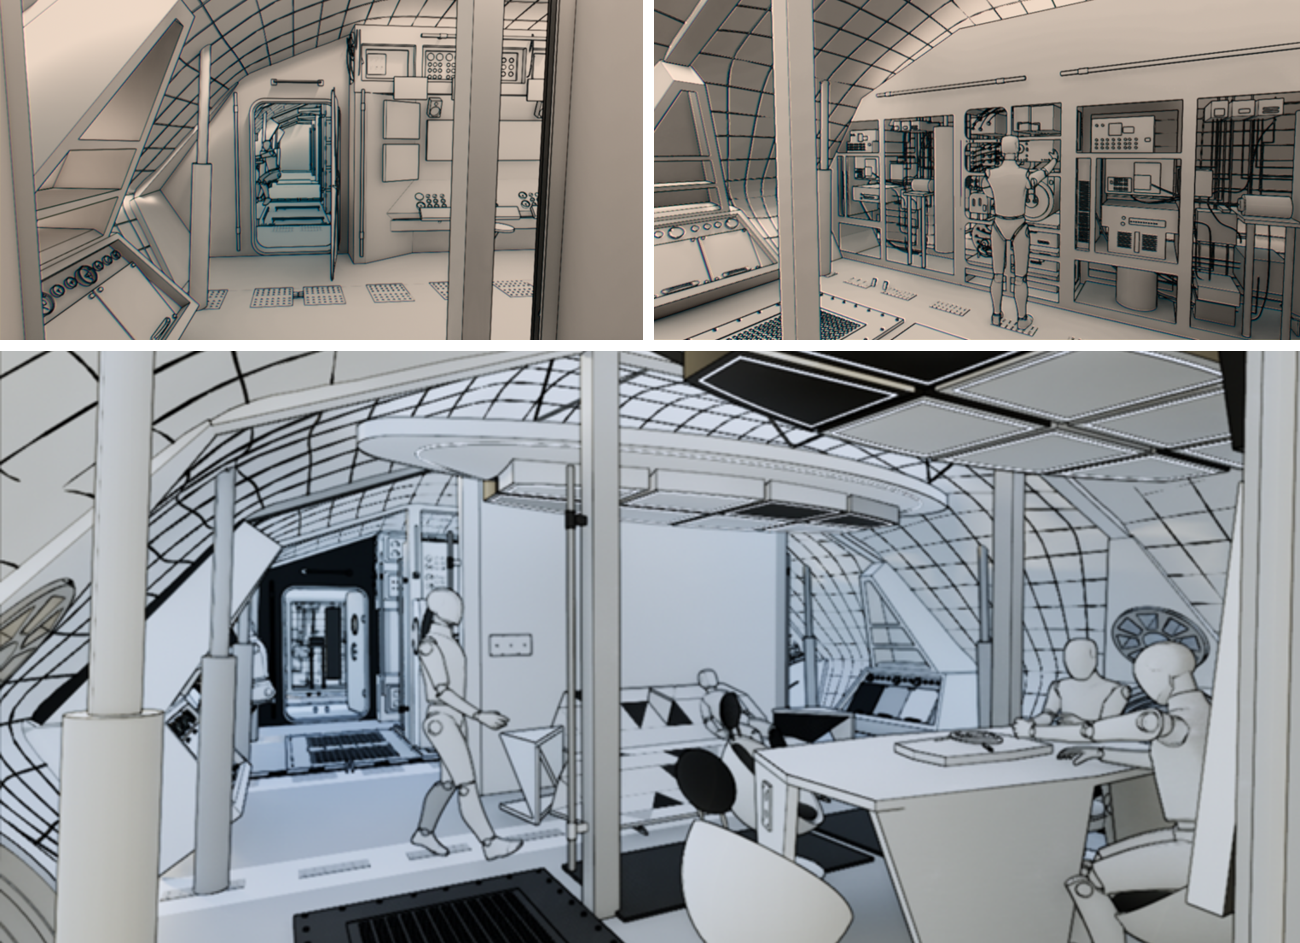
\includegraphics[scale=0.7]{images/calpoly_vr.png}

\paragraph{A marsjárón biztosítani kell maximum négy ember 20 napnyi összkomfortos komfortfokozatú életterét.}


\begin{description}
\item[összkomfortos] Az a lakás, amely legalább egy 12 $m^2$-t meghaladó alapterületű lakószobával, főzőhelyiséggel, fürdőhelyiséggel és WC-vel, valamint közművesítettséggel, melegvíz-ellátással és központos fűtési móddal rendelkezik. 
\end{description}

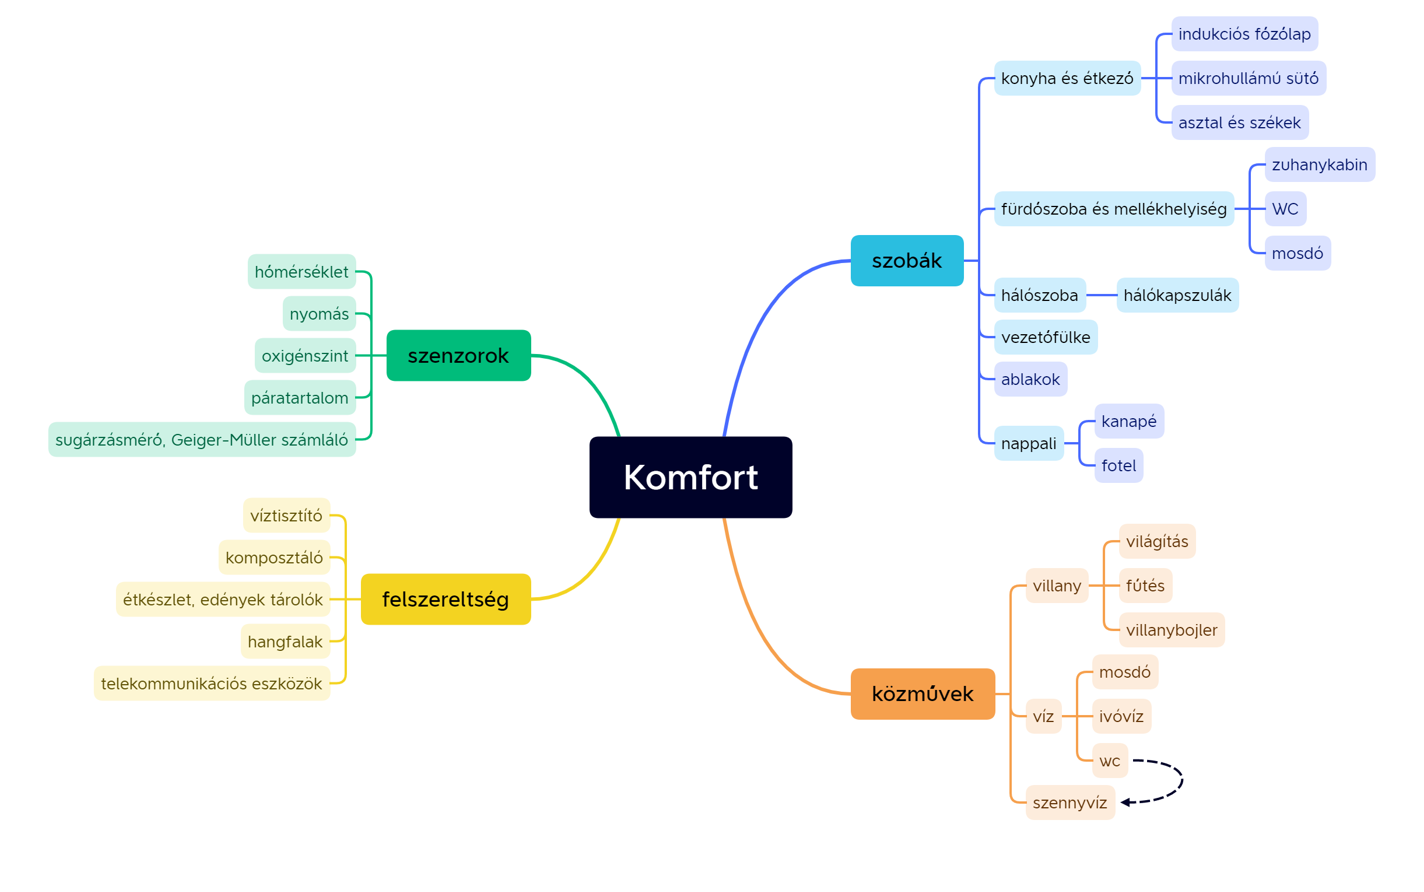
\includegraphics[scale=0.4]{images/komfort01.png}

A fenti ábrán látható öt szobára  van szükség a legénység életterének biztosításához a belmagasság 2.2m 300 lumen megvilágítással. \\(\reqid{KO_1}) vezetőfülke 3m x 2m alapterületű, melyben két ülés található. Az üléseken állítható a fejtámla, a háttámla, az ülésmagasság, a kartámla magassága és szöge. Az ülés 1.7m x 0.8m x 0.65m méter. \\(\reqid{KO_2}) Fürdőszoba és mellékhelyiség 2m x 4m alapterületű, melyekben egy 0.75m x 0.75m alapterületű zuhanykabin helyezkedik el, valamint egy öblítéses wc és mosdókagyló. Mindkét elfolyást egy tisztító rendszerbe vezetjük el, víz visszanyerés céljából. 20 napnyi tisztálkodáshoz és szükségletek elvégzéséhez szükséges felszerelést egy 0.5m x 0.3m alapterületű falhoz rögzített szekrényben tároljuk.  \\(\reqid{KO_3}) Konyha és étkező 25 nm alapterületű. Egy ember napi 3 liter vízfogyasztással számolva 4 ember x 3liter x 20 nap = 240 l (minimum) tárolására alkalmas, mivel nagyrészét elő tudjuk állítani így 80 liter fogyasztásra kész szobahőmérséklető ivóvíztartály. 

Konyha felszereltsége:
\begin{itemize}
    \item hűtőszekrény: mivel a Marson az átlaghőmérséklet $ -63^\circ C $ ezért a hűtésre fordított energiát a Mars légköréből biztosítják, hogy kevesebb kompressziós energiával lehessen a hűtést megoldani.
    \item indukciós főzőlap
    \item mosogatógép
    \item egyéb konyhai eszközök (mikrohullámú sütő, robotgép, edények) tárolására alkalmas szekrény
    \item evőeszközök: 4 pár étkészlet 4 darab pohár és bögre
    \item szelektív hulladék gyűjtésére kialakított tárolók
    \item mosó és szárítógép
\end{itemize}

(\reqid{KO_4}) Nappali, egy 3m x 4m alapterületű közösségi helység, melyben két darab egyszemélyes (állítható a fejtámla, a háttámla, az ülésmagasság, a kartámla magassága és szöge de a szék rögzítve van a padlóhoz) valamint egy kétszemélyes falhoz és padlóhoz rögzített 1.5m x 0.8m x 0.7m kanapé található -- minden bútoron biztonsági öv vihar esetére. A székek a kanapéval szemben helyezkednek el köztük egy 0.4m x 1m állítható magasságú asztallal. A szobában általános elsősegély csomag és defibrillátor a falra felszerelve található, alatta \ce{CO2} tűzoltó készülék.\\(\reqid{KO_5}) Hálószoba 3m x 4m területű melyben falhoz rögzített négy darab 0.4m x 0.3m belmagasságig érő ruhásszekrény a legénység számára és  2 db (2m*0.5m*0.4m) hálókapszula található

A marsjáróban állandó oxigénszint, hőmérséklet, páratartalom, lég, hangnyomás és sugárzásmérő kell vagyis az alábbi szenzorok szükségesek:

Szenzorok:
\begin{itemize}
    \item (\reqid{KO_6}) hőmérséklet: $22^\circ C $ 
    \item (\reqid{KO_7})páratartalom: 40-60 \%
    \item (\reqid{KO_8})oxigénszintmérő (lsd feljesbb humánkövetelmények)
    \item (\reqid{KO_9})légnyomásmérő: 1013,25 hPa
    \item (\reqid{KO_10})sugárzásmérő (külső és belső, hogy a kozmikus sugárzás ne veszélyeztessen emberéletet)
    \item (\reqid{KO_11})dB mérő: 30-60 dB biztosítása (megfelelő hangszigetelés a külső zajok kiszűrésére
\end{itemize}


\section{Biztonsági követelmények}

A biztonságos misszióhoz elengedhetetlen a jármű kockázat analaízise, mely során annak alrendszereit feltérképezzük és a kritikusakat meghatározzuk. 

\subsection{Kockázat analízis}

A kockázat analízis célja, hogy a \ref{subsystems} fejezetben részletezett alrendszerek közül melyek a kritkus rendszerek és mennyire fontosak. A legnyílvánvalóbb az energia ellátó alrendszer, hiszen ha nincsen enerigai hiába van létfentartó rendszer vagy bármi más. Ha nincsen energia, akkor nem várható el egyik alrendszertől, vagy tartalékrendszertől sem, hogy működjön.

Miután a járműnek van redundás energiaforrása, a létfenntartó rendszert fontos megvizsgálni. Az tényként kezelendő, hogy a fedélzeten utazó űrhajósokat életben kell tartni, így ezen rendszereknek is szükséges tartalékot képezni, legalább a levegő- és vízkezelés illetve a fűtés szintjén. 

\textit{Megjegyzés: A rover tartalékrendszerein túl az utasok bármikor felvehetik a szkafander sisakjukat, így akár egy harmadfokú renduncacnia is elérhető.}

A fent említett rendszereken túl, a harmadik a sorban a telekommunkációs rendszerek, hogy a kutatók tudjanak segítséget kérni a bázistól, vagy a másik rovertól amennyiben szükséges.

\begin{itemize}
  \item Az esetleges katasztrófaesemények esetén is biztosítani kell a személyzet, bázisra való visszajutását.
\end{itemize}
\section{Utókövetelmények}
\begin{itemize}
  \item \reqid{U_1} A marsjáró leszerelése és kezelése mint hulladék.
  \item \reqid{U_2} A marsjáró által okozott esetleges természeti károk helyreállítási terve.
\end{itemize}

\chapter{Szójegyzék}
\section{Marsi fogalmak}
\begin{itemize}
  \item A marsi gravitáció 3.721 m/s².
  \item A marsi év 687 nap. A fentiekben mi földi évben számolunk.
  \item A mars átlaghömérséklete -62°C. -120°C és +20°C között ingadozik.
  \item A marsi UV sugárzás $\approx$50 W/m². Ez a földi átlagnál körülbelül 5-ször nagyobb, ami az eszközök élettartamát befolyásolja.
\end{itemize}


\section{További fogalmak}

\begin{itemize}

  \item \textbf{misszió}: Latin \textit{missio} szóból ered. Jelentése: küldetés.
  \item \textbf{drón}: Hivatalosabban pilóta nélküli légijárműveknek (UAV) vagy pilóta nélküli repülőgép-rendszereknek nevezik. Távirányítással vagy önállóan képes repülni a beágyazott rendszereiben található szoftvervezérelt repülési tervek segítségével.
  \item \textbf{giroszkóp}: A tájolás és a szögsebesség mérésére vagy fenntartására használt eszköz.
  \item \textbf{detektálás}: észlelés, érzékelés, felfedezés
  \item \textbf{szenzor}: érzékelő műszer, eszköz
  \item \textbf{szkafander}: Eredete az orosz \textit{szkafandr} szó. Jelentése: űrruha.
  \item \textbf{koaxiális propellerek}: Egy tengelyen egymás fölött elhelyezett két darab propeller, amik ellentétes irányba forognak. Ezzel nagyban javul a hajtás és manőverezés.
  \item \textbf{propeller}: Légcsavar. Repülőgépek, helikopterek és egyéb repülő eszközök (ezesetben drón) körében használt erőátviteli megoldás. A motor teljesítményét közvetíti a hordozó közegre (levegő).
  \item \textbf{FIFO módszer}: "First in first out", azaz amelyik adat (képfelvétel) előszür került tárolásra azt továbbítja / az vehető ki először.
  \item \textbf{regolit}: Szilárd kérgű égitesteken a felszíni törmelékes, általában laza szerkezetű kőzetrétege. A talaj is a regolitnak nevezhető, de regolitról leginkább akkor beszélünk, ha a regolitréteg nem talajosodott.
  \item \textbf{geológia}: földtan
  \item \textbf{hőpárologtatás}: a kiásott lyuk mélyére egy hevítőrudat juttatnak, a hő hatására a kőzetben reakciók hajtódnak végre, anyagok válnak ki, amelyek vizsgálatával fontos információhoz juthatunk
  \item \textbf{UHF}: Ultra High Frequency, vagyis ultramagas frekevincia. 300 MHz és 3 GHz közötti tartomány.
\end{itemize}


\end{document}
